\documentclass{report}
\usepackage[spanish]{babel}

\usepackage[most,many,breakable]{tcolorbox}
\usepackage{xcolor}

\definecolor{defBoxBorder}{HTML}{395144}
\newtcolorbox{defBox}{colback=white,colframe=defBoxBorder,arc=3pt, boxrule=0.5pt, drop fuzzy shadow, title=Definition}
\definecolor{thBoxBorder}{HTML}{AC8441}
\newtcolorbox{thBox}{colback=white,colframe=thBoxBorder,arc=3pt, boxrule=0.5pt, drop fuzzy shadow, title=Theorem}
\definecolor{noteBoxBorder}{HTML}{4E6C50}
\newtcolorbox{noteBox}{colback=white,colframe=noteBoxBorder,arc=3pt, boxrule=0.5pt, drop fuzzy shadow, title=Note}
\definecolor{axBoxBorder}{HTML}{AA5656}
\newtcolorbox{axBox}{colback=white,colframe=axBoxBorder,arc=3pt, boxrule=0.5pt, drop fuzzy shadow, title=Axiom/Postulate}
\definecolor{corBoxBorder}{HTML}{8B7E74}
\newtcolorbox{corBox}{colback=white,colframe=corBoxBorder,arc=3pt, boxrule=0.5pt, drop fuzzy shadow, title=Corollary}
\definecolor{lemBoxBorder}{HTML}{B99B6B}
\newtcolorbox{lemBox}{colback=white,colframe=lemBoxBorder,arc=3pt, boxrule=0.5pt, drop fuzzy shadow, title=Lemma}


\usepackage[spanish]{babel}
\usepackage[utf8x]{inputenc}
\usepackage{amsmath}
\usepackage{graphicx}
\usepackage[colorinlistoftodos]{todonotes}
\usepackage{enumitem}
\usepackage{listings}
\usepackage{verbatim}
\usepackage{eurosym}
\usepackage[export]{adjustbox}
\usepackage{amssymb}
\usepackage{bussproofs}
\usepackage{amsmath}
\usepackage{tikz}
\usepackage{xcolor}
\usepackage{listings}
\usepackage{titletoc}
\usepackage{hyperref}

\hypersetup{
  colorlinks=true,
  linkcolor=black,
  urlcolor=blue,
  citecolor=black
}

\newcommand{\coverPage}[6]{%
%----------------------------------------------------------------------------------------
%	COVER START
%----------------------------------------------------------------------------------------
\begin{titlepage}

    \newcommand{\HRule}{\rule{\linewidth}{0.5mm}}
    \newcommand{\department}{#1}
    \newcommand{\course}{#2}
    \newcommand{\titleValue}{#3}
    \newcommand{\subtitleValue}{#4}
    \newcommand{\authorName}{#5}

    \center

    %----------------------------------------------------------------------------------------
    %	HEADER
    %----------------------------------------------------------------------------------------
    
\includegraphics{images/logo_usa.png}
    \vspace{0.5cm}
    \textsc{\Large \department}\\[0.5cm]
    \textsc{\Large \course}\\[0.5cm]
    \vfill

    %----------------------------------------------------------------------------------------
    %	TITLE
    %----------------------------------------------------------------------------------------

    \HRule\\
    \Huge
    \textbf{\titleValue}\\[0.5cm]
    \Large
    \textbf{\subtitleValue}\\
    \HRule\\[0.5cm]

    %----------------------------------------------------------------------------------------
    %	AUTHOR AND DATE
    %----------------------------------------------------------------------------------------

    \vfill
    \Large
    \textit{\authorName}\\
    {\large \today}\\[2cm]

\end{titlepage}
%----------------------------------------------------------------------------------------
%	COVER END
%----------------------------------------------------------------------------------------
}

\begin{document}
    \coverPage{ Matemáticas }{ Cálculo Integral y Series }{ Integrabilidad }{  }{ Alexander Mendoza }{\today}
    \tableofcontents

    \chapter*{Prólogo}
    Después de visitar el curso introductorio de Cálculo infinitesimal, Cálculo diferencial, ahora continuaremos con el curso que liberará todo el potencial de la derivada, Cálculo Integral. En esta primera parte del curso comenzaremos dando una idea intuitiva de lo que es la integral, planteando los problemas que la originaron. Luego definiremos formalmente la integral de una función y afirmaremos sus propiedades para encontrar fácilmente su valor. Y, finalmente, proporcionaremos el teorema que unifica Cálculo diferencial e integral, creando así una relación entre la integral y la derivada de una función.

    \pagebreak
    \chapter{Integrabilidad}
    La principal motivación de la integral fue tener una forma de calcular el área bajo una curva. Por ejemplo, si tuvieras un barril sin fondo, querrías saber cuánta madera necesitarías para repararlo. El primer intento conocido para abordar este problema fue presentado por los matemáticos griegos y se llamaba el método de agotamiento. El método consistía en dar una región, llenarla con una secuencia de figuras polinómicas hasta llenar el área.

    \begin{Figure}
        \begin{center}
        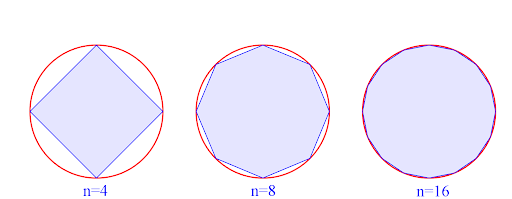
\includegraphics[width=1\textwidth]{images/exhaustion.png}
        \end{center}
    \end{Figure}

    Antes de definir formalmente la integral, primero necesitaremos algunas definiciones.
    \section{Sumas inferiores y superiores}
    Usaremos tanto las sumas superiores como las inferiores para definir el concepto de integral.

    \begin{defBox}
        \textit{\textbf{Partición de una integral.}} Sean $a$ y $b$ números reales tales que $a<b$ y sea $P$ el siguiente conjunto

        $$P = \{x_0, x_1, \dots , x_n\}$$ con $a=x_0<x_1<\cdots<x_n=b$, entonces decimos que $P$ es una partición de $[a,b]$.
    \end{defBox}

    El concepto de partición se puede ver simplemente como dividir el intervalo en intervalos más pequeños y guardarlos dentro de un conjunto.
    \begin{Figure}
        \begin{center}
            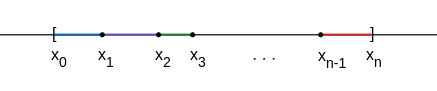
\includegraphics[width=1\textwidth]{images/partitions2.png}
        \end{center}
    \end{Figure}
    La Figura 1.1.2 representa gráficamente el concepto de partición de un intervalo. Cada parte coloreada es un segmento de la partición y hay que notar cómo la definición no requiere que la longitud de los segmentos sea igual.

    \begin{Example}
        Consideremos el intervalo $S = [-1, 6]$, entonces el conjunto $\{0, \sqrt{2}, \frac{3}{2}, 4, 5\}$ sería una partición de $S$.
    \end{Example}
    \begin{defBox}
        \textit{\textbf{Mínimo y máximo}}. Sea $f$ una función acotada en $[a,b]$ y sea $P = \{x_0, x_1, \dots x_n\}$ una partición de $[a,b]$. Entonces

        El mínimo de una función en $[a,b]$ se define como
        $$m_i := inf\{f(x) | x_{i-1} \leq x \leq x_i\}$$
        Y el máximo de una función en $[a,b]$ se define como
        $$M_i := sup\{f(x) | x_{i-1} \leq x \leq x_i\}$$
    \end{defBox}

    % Add examples

    \begin{Example}
        Consideremos la función $$f(x) =
        \begin{cases}
        x^2 & \text{si } 0 \leq x < 1 \\
        1.5 & \text{si } 1 \leq x \leq 3 \\
        -1.5(x-5) & \text{si } 3 < x \leq 5
        \end{cases}$$
        Junto con el intervalo $[0, 5]$ y la partición $P = \{\frac{1}{2}, \frac{3}{2}\}$

        \begin{center}
            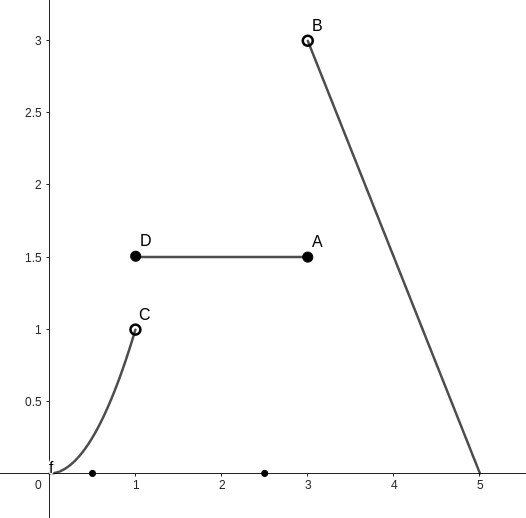
\includegraphics[width=.5\textwidth]{images/minmax.png}
        \end{center}

        Entonces la tabla de valores mínimos y máximos sería la siguiente

        \begin{center}
            \begin{table}[h]
                \begin{tabular}{l|l|l|l}
                    $i$ & $[x_{i-1}, x_i]$             & $m_i$         & $M_i$         \\ \hline
                    1   & $[0, \frac{1}{2}]$           & 0             & $\frac{1}{4}$ \\
                    2   & $[\frac{1}{2}, \frac{5}{2}]$ & $\frac{1}{4}$ & $\frac{3}{2}$ \\
                    3   & $[\frac{5}{2}, 5]$           & 0             & 3
                \end{tabular}
            \end{table}
        \end{center}

    \end{Example}

    Con esto ya podemos definir las sumas inferiores y superiores.

    \begin{defBox}
        Supongamos que $f$ está acotada en $[a,b]$, sea $P = \{t_0,\dots,t_n\}$ una partición de $[a,b]$ y sea

        $$m_i = inf\{f(x) | x_{i-1} \leq x \leq x_i\}$$
        $$M_i = sup\{f(x) | x_{i-1} \leq x \leq x_i\}$$

        Luego definimos la suma inferior de $f$ para $P$, denotada por $L(f, P)$, como

        $$L(f, P) = \sum_{i=1}^{n}m_i(t_{i} - t_{i-1})$$

        y la suma superior de $f$ para $P$, denotada por $U(f, P)$, se define como

        $$U(f, P) = \sum_{i=1}^{n}M_i(t_{i} - t_{i-1})$$
    \end{defBox}

    Las sumas inferiores y superiores se pueden visualizar como

    \begin{Figure}
        \begin{center}
        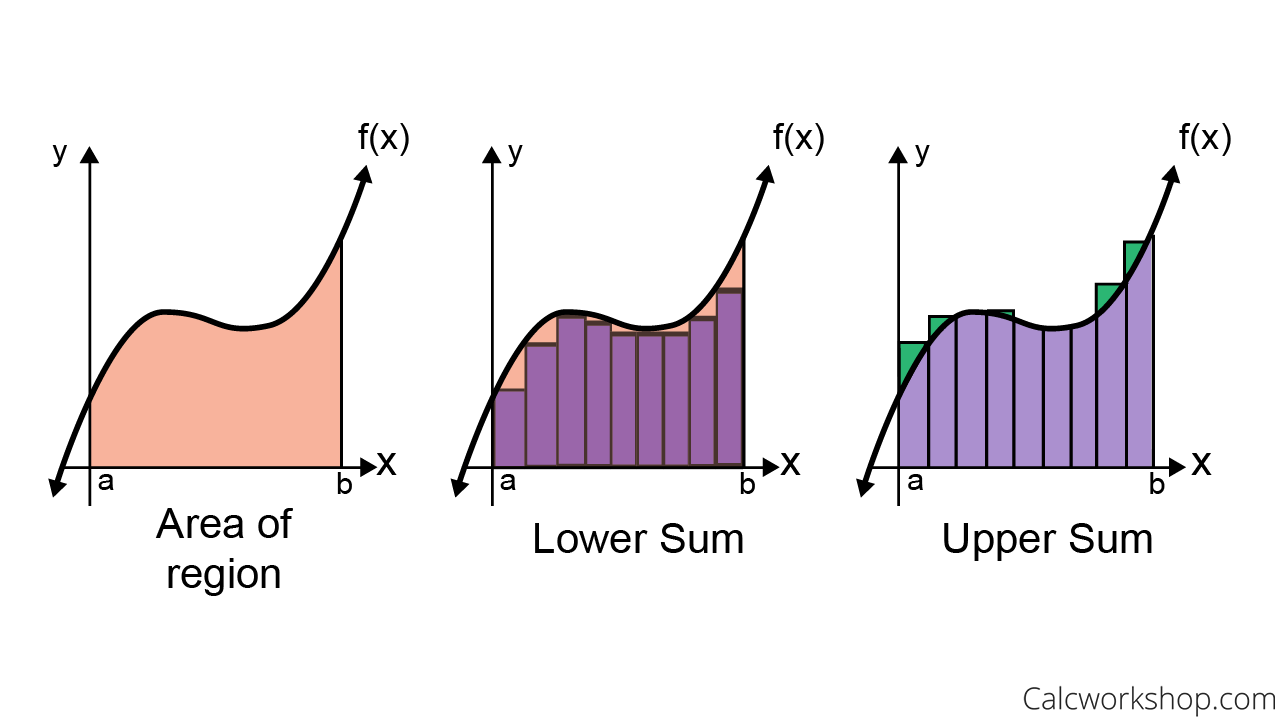
\includegraphics[width=1\textwidth]{images/lowerupper.png}
        \end{center}
    \end{Figure}

    \textbf{Función:} \( f(x) = x^2 \) en el intervalo \( [0, 2] \) con partición \( P = \{0, \frac{1}{2}, 1, \frac{3}{2}, 2\} \)

    \textbf{Suma inferior:}
    \[
    L(f, P) = 0 \times \frac{1}{2} + \frac{1}{4} \times \frac{1}{2} + 1 \times \frac{1}{2} + \frac{9}{4} \times \frac{1}{2} = 2
    \]

    \textbf{Suma superior:}

    \[
    U(f, P) = \frac{1}{4} \times \frac{1}{2} + 1 \times \frac{1}{2} + \frac{9}{4} \times \frac{1}{2} + 4 \times \frac{1}{2} = \frac{17}{4}
    \]

    Ahora veamos qué relación tienen la suma inferior y la suma superior. Nuestra intuición puede decirnos que dado $f$ acotada sobre $[a,b]$ y $P$ una partición de $[a,b]$, $L(f, P) \leq U(f, P)$, de hecho esto es cierto para cada par de particiones distintas. Pero, repasemos primero un lema para demostrar este hecho.

    \begin{lemBox}
        Sean $f$ una función acotada y $P, Q$ particiones de $[a,b]$. Si $Q \subseteq P$, entonces

        $$L(f, Q) \leq L(f, P) $$
        $$U(f, P) \leq U(f, Q) $$
    \end{lemBox}

    \begin{ideaBox}
        La idea de esta prueba es demostrar primero que el lema es cierto para una partición $Q$ que contiene solo un elemento más que una partición $P$, y luego construir una secuencia de particiones, donde cada nueva partición tenga un elemento más que la partición anterior, y probar el caso general.
    \end{ideaBox}

    \textit{\textbf{Prueba.}}
    \noindent\textbf{Primera parte de la prueba}
    Sea $f$ una función acotada en $[a,b]$ y sean $P, Q$ particiones de $[a,b]$ donde $Q \subseteq P$ y $P$ contiene solo un elemento más que $Q$, a saber, $u$. Podemos representar $P$ y $Q$ como

    $$P = \{x_0,x_1,\dots,x_{k-1},x_k,\dots,x_n\}$$
    $$Q = \{x_0,x_1,\dots,x_{k-1},u,x_k,\dots,x_n\}$$

    Luego sea

    $$m' = inf\{f(x) | t_{k-1} \leq x \leq u\}$$
    $$m'' = inf\{f(x) | u \leq x \leq t_k\}$$

    Y por definición de suma inferior tenemos

    \begin{align*}
        L(f,P) &= \sum_{i=1}^{n} m_i(x_i-x_{i-1})\\
        &= \left(\sum_{i=1}^{k-1}m_i(x_i-x_{i-1})\right) \\
        &+ m_k(x_k-x_{k-1}) \\
        &+ \left(\sum_{i=k+1}^{n}m_i(x_i-x_{i-1})\right)
    \end{align*}

    De manera similar

    \begin{align*}
        L(f,Q) &= \sum_{i=1}^{n} m_i(x_i-x_{i-1})\\
        &= \left(\sum_{i=1}^{k-1}m_i(x_i-x_{i-1})\right)\\
        &+ m'(u-x_{k-1}) + m''(x_k-u)\\
        &+ \left(\sum_{i=k+1}^{n}m_i(x_i-x_{i-1})\right)
    \end{align*}

    Con esto, sería suficiente mostrar que $m_k(t_k-t_{k-1}) \leq m'(u - t_{k-1}) + m''(t_k-u)$. Sabemos que $m_k \leq m'$, esto porque $\{f(x) | t_{k-1} \leq x \leq u\} \subseteq \{f(x) | t_{k-1} \leq x \leq t_k\}$, por lo tanto, este último conjunto contiene todos los elementos del primero y puede contener elementos más pequeños. Un razonamiento similar se puede hacer para concluir $m_k \leq m''$. Entonces tenemos

    \begin{align*}
        m_k(t_k-t_{k-1}) &= m_k(t_k+0-t_{k-1})\\
        &= m_k(t_k+(-u+u)-t_{k-1})\\
        &= m_k((t_k-u)+(u-t_{k-1}))\\
        &= m_k(t_k-u)+m_k(u-t_{k-1})\\
        &\leq m''(t_k-u) + m'(u-t_{k-1}) &&\text{ Esto debido a las propiedades de la desigualdad.}
    \end{align*}
    Por lo tanto, $L(f,P) \leq L(f, Q)$. La prueba para la suma superior es análoga.\\

    \noindent\textbf{Segunda parte de la prueba}

    Supongamos que $Q$ contiene $m$ puntos más que $P$. Luego creamos una secuencia de particiones para $[a,b]$, $\{P = P_0, P_1, P_2, \dots , P_m = Q\}$ donde $P = P_0 \subseteq P_1 \subseteq P_2 \subseteq \dots \subseteq P_m = Q$ y $P_i$ contiene un punto más que $P_{i-1}$, entonces por la primera parte de la prueba

    $$L(f,P) \leq L(f,P_1) \leq L(f,P_2) \leq \cdots \leq L(f,Q)$$

    Por transitividad, por lo tanto tenemos $L(f,P) \leq L(f,Q)$. Usando un razonamiento similar tenemos $U(f,P) \geq U(f,Q)$. Concluyendo nuestra prueba.\\

    Otra observación útil es la siguiente

    \begin{lemBox}
        Dada cualquier partición $P$
        $$L(f, P) \leq U(f, P)$$
    \end{lemBox}
    \textit{\textbf{Prueba}}. Sabemos esto porque
    $$L(f, P) = \sum_{i=1}^{n}m_i(t_{i} - t_{i-1})$$
    $$U(f, P) = \sum_{i=1}^{n}M_i(t_{i} - t_{i-1})$$
    y por definición, para cualquier $i$:
    \begin{align*}
        m_i &\leq M_i\\
        m_i(t_{i} - t_{i-1}) &\leq M_i(t_{i} - t_{i-1})
    \end{align*}

    \begin{thBox}
        Sea $P_1, P_2$ una partición de un intervalo $[a,b]$ y sea $f$ acotada en $[a,b]$, entonces es cierto que

        $$L(f, P_1) \leq U(f, P_2)$$
    \end{thBox}

    \textit{\textbf{Prueba.}} Sea $P = P_1 \cup P_2$, luego por el lema 1.1.8 tenemos las siguientes desigualdades:
    \begin{align}
        L(f, P'') &\leq L(f, P)\\
        U(f, P') &\geq U(f, P)
    \end{align}
    Multiplicando la desigualdad 1.3 por $-1$ y sumándola a la desigualdad $1.4$ obtenemos:
    $$
        L(f, P) \leq U(f, P)
    $$

    Y en conjunto, obtenemos:
    $$
        L(f, P'') \leq L(f, P) \leq U(f, P) \leq U(f, P')
    $$

    Por transitividad, por lo tanto, tenemos:
    $$
        L(f, P'') \leq U(f, P')
    $$

    En consecuencia, $L(f, P'') \leq U(f, P')$. Concluyendo nuestra prueba.

    \begin{Example}
        Sea $f(x) = C$ una función acotada en $[a,b]$ para alguna constante $C$. Luego $C = m_i = M_i$ para cualquier partición $P$ en $[a,b]$. Entonces
        $L(f, P) = U(f, P) = C(b-a)$

        Por lo tanto, tenemos
        $$\sup\{L(f, P)\} = \inf\{U(f, P)\}$$

        Por lo tanto, $f$ es integrable en $[a,b]$ y $\int_{b}^{a}f = C(b-a)$. Esta sería la fórmula para un rectángulo. Gráficamente:

        \begin{center}
            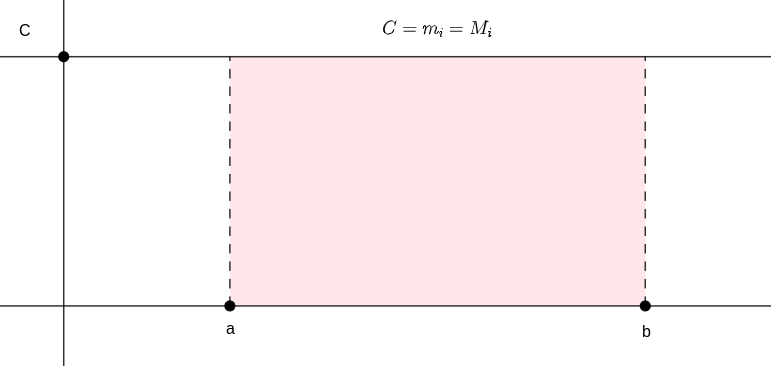
\includegraphics[width=1\textwidth]{images/integralconstant.png}
        \end{center}
    \end{Example}

    \begin{Example}
        Sea $$f(x) =
        \begin{cases}
        1 & \text{si } x \text{ es racional} \\
        0 & \text{si } x \text{ es irracional}
        \end{cases}$$
        una función acotada en el intervalo $[0,1]$

        Sabemos que para cualquier partición $P$, $m_i = 0$ y $M_i = 1$. Entonces
        $$ L(f, P) = 0 \neq U(f, P) = 1$$

        Por lo tanto
        $$\sup\{L(f, P)\} \neq \inf\{U(f, P)\}$$

        y, por lo tanto, $f$ no es integrable en $[0,1]$.
    \end{Example}

    \section{Criterio para la integrabilidad}
    Ahora que sabemos cómo saber si la integral de una función existe, necesitamos una forma más fácil de encontrar el valor de la integral.

    \begin{thBox}
        \textit{\textbf{Criterio para la Integrabilidad}}. Si $f$ está acotada en $[a,b]$, entonces $f$ es integrable en $[a,b]$ si y solo si, para cada $\epsilon > 0$ hay una partición $P$ de $[a,b]$ tal que
        $$U(f,P)- L(f,P) < \epsilon$$
    \end{thBox}

    \begin{noteBox}
        Durante la prueba usaremos el hecho de que $a-b < \epsilon$ para cualquier $\epsilon > 0$ implica que $a = b$. Esto se puede comprobar utilizando la propiedad arquimediana de los números reales de la siguiente manera:\\

        Supongamos que $a \neq b$, entonces $a-b > 0$, por la propiedad arquimediana, existe un número $n$ tal que

        $$a-b > \frac{1}{n}$$

        Esto significa que dado $\epsilon = 1/n$, $a-b>\epsilon$, lo cual contradice nuestra premisa. Por lo tanto, $a=b$.
    \end{noteBox}

    \textit{\textbf{Prueba.}} Comencemos con la primera implicación de la prueba. Supongamos que para todo $\epsilon > 0$ hay una partición $P$ de $[a,b]$ tal que $U(f, P) - L(f, P) < \epsilon$ y sea $\mathcal{P}$ el conjunto de todas las particiones de $[a,b]$, a partir de esto obtenemos las siguientes desigualdades:
    \begin{align}
        \sup\{L(f, Q) | Q \in \mathcal{P}\} &\geq L(f,P)\\
        \inf\{U(f, Q) | Q \in \mathcal{P}\} &\leq U(f,P)
    \end{align}

    Multiplicando la desigualdad 1.1 por $-1$ y sumándola a la desigualdad $1.2$ obtenemos:
    $$
        \sup\{L(f, Q) | Q \in \mathcal{P}\} - \inf\{U(f, Q) | Q \in \mathcal{P}\} \leq U(f,P) - L(f,P)
    $$

    Esto implica:
    $$
        \sup\{L(f, Q) | Q \in \mathcal{P}\} - \inf\{U(f, Q) | Q \in \mathcal{P}\} < \epsilon
    $$

    Y por lo tanto $\sup\{L(f, Q) | Q \in \mathcal{P}\} = \inf\{U(f, Q) | Q \in \mathcal{P}\}$.\\

    A la inversa, supongamos ahora que $f$ es integrable en $[a,b]$, es decir,
    $$\sup\{L(f, Q) | Q \in \mathcal{P}\} = \inf\{U(f, Q) | Q \in \mathcal{P}\}$$
    Entonces hay $P', P'' \in \mathcal{P}$ tal que
    $$ U(f, P'') - L(f, P') < \epsilon$$
    para todo $\epsilon > 0$. Si esto no fuera cierto, encontraríamos una contradicción debido a las definiciones de supremo e ínfimo.

    Ahora, sea $P = P' \cup P''$, luego por el lema 1.1.8 tenemos las siguientes desigualdades:
    \begin{align}
        L(f, P'') &\leq L(f, P)\\
        U(f, P') &\geq U(f, P)
    \end{align}
    y multiplicando la desigualdad 1.3 por $-1$ y sumándola a la desigualdad 1.4 obtenemos
    $$U(f,P)-L(f, P) \leq U(f, P') - L(f, P'') < \epsilon$$

    Y, por lo tanto, $U(f,P)-L(f, P) < \epsilon$.

    \begin{Example}
        Sean $f(x) = x$ donde $x \in [0,b]$, entonces tenemos $m_i = x_{i-1}$ y $M_i = x_i$. Entonces, por definición sabemos que:

        \begin{align*}
            L(f, P) &= \sum_{i=1}^{n} m_{i}(x_{i} - x_{i-1})\\
            &= \sum_{i=1}^{n}x_{i-1}(x_{i} - x_{i-1})
        \end{align*}
        De manera similar:
        $$U(f, P) = \sum_{i=1}^{n}x_{i}(x_{i} - x_{i-1})$$

        Entonces

        \begin{align*}
            U(f, P)- L(f, P) &= \sum_{i=1}^{n} \left[x_i(x_i-x_{i-1}) - x_{i-1}(x_i-x_{i-1})\right]\\
            &= \sum_{i=1}^{n} \left[(x_i-x_{i-1})(x_i-x_{i-1})\right]\\
            &= \sum_{i=1}^{n} (x_i-x_{i-1})^2
        \end{align*}

        Ahora, sea $P_n$ una partición de $[0,b]$ tal que $x_i - x_{i-1} = \frac{b-a}{n} = \frac{b-0}{n} = \frac{b}{n}$, entonces:

        \begin{align*}
            U(f, P)- L(f, P) &= \sum_{i=1}^{n} \left(\frac{b}{n}\right)^2\\
            &= \frac{b^2}{n}
        \end{align*}

        Ahora, dado $\epsilon > 0$ sea $P_n$ la partición previamente definida de $[0,b]$ con $n > \frac{b^2}{\epsilon}$ de manera que:

        $$U(f, P)- L(f, P) = \frac{b^2}{n} < \epsilon$$

        Por lo tanto, $f$ es integrable.

        % COMPLETAR LA PRUEBA PARA EL VALOR DE LA INTEGRAL
    \end{Example}

    % INSERTAR EL EJEMPLO PARA x^2

    \section{Continuidad uniforme}

    Ahora definiremos un concepto que nos ayudará a proporcionar un teorema que facilitará determinar si una función es integrable o no.

    \begin{noteBox}
        Recordemos que la definición estándar de continuidad es la siguiente:

        $f$ es continua en un punto $a$ si y solo si, para cada $\epsilon > 0$, existe $\delta > 0$ tal que para todo $x$, si $|x-a|<\delta$, entonces $|f(x) -f(a)| < \epsilon$.
    \end{noteBox}
    \begin{defBox}
        \textit{\textbf{Continuidad uniforme}}. $f$ es uniformemente continua en un intervalo $A$ si y solo si, para todo $\epsilon > 0$ existe $\delta > 0$ tal que para todo $x, y \in A$, si $|x-y| < \delta$, entonces $|f(x) - f(y)| < \epsilon$
    \end{defBox}

    Esta definición se puede interpretar de la siguiente manera, cuando ocurren cambios pequeños en $x$, producen cambios pequeños en $f(x)$, pero tales cambios en $f(x)$ no dependen del valor de $x$.

    % INSERT EXAMPLES FOR UNIFORM CONTINUITY

    Sabiendo esto, enunciaremos algunos teoremas que nos ayudarán a probar que una función continua es integrable.

    \begin{thBox}
        Si $f$ es uniformemente continua en un intervalo $I$, entonces $f$ es continua en $I$
    \end{thBox}

    \begin{thBox}
        \textit{\textbf{Teorema de Heine-Cantor}}. Si $f$ es continua en $[a,b]$, entonces $f$ es uniformemente continua en $[a,b]$
    \end{thBox}

    \begin{thBox}
        Si $f$ es continua en $[a,b]$, entonces $f$ es integrable en $[a,b]$
    \end{thBox}

    % COMPLETE THE PROOF

    \section{Álgebra de integrales}

    Hasta ahora hemos enunciado algunos teoremas teóricos. Ahora revisemos algunos teoremas operativos.

    \begin{thBox}
        $f$ es integrable en $[a,b]$ si y solo si, $f$ es integrable en $[a,c]$ y en $[c,b]$. Además:

        $$\int_{a}^{b}f = \int_{a}^{c}f + \int_{c}^{b}g$$
    \end{thBox}

    % \begin{ideaBox}
    %     La idea de la prueba es seleccionar una partición donde uno de los elementos de la partición sea $c$, luego crear dos particiones más, una a partir de 
    % \end{ideaBox}

    \textit{\textbf{Prueba.}} Supongamos que $f$ es integrable en $[a,b]$. Entonces

    \begin{thBox}
        Si $f$ y $g$ son integrables en $[a,b]$, entonces $f+g$ es integrable. Además:

        $$\int_{a}^{b}f+g = \int_{a}^{b}f + \int_{a}^{b}g$$
    \end{thBox}

    \begin{defBox}
        $$\int_{a}^{a}f = 0$$;
        $$\int_{a}^{b}f = - \int_{b}^{a}f \text{ si } a> b$$
    \end{defBox}

    \begin{thBox}
        Si $f$ es integrable en $[a,b]$ y $m\leq f(x) \leq M$ para todo $x \in [a,b]$, entonces:

        $$m(b-a) \leq \int_{a}^{b}f \leq M(b-a)$$
    \end{thBox}

    % INSERT EXAMPLES ABOUT INTEGRABLE FUNCTIONS

    \section{El Teorema Fundamental del Cálculo}

    Después de definir la integral, utilizando un método no muy intuitivo; encontrar un criterio para la integrabilidad, que facilita el proceso de encontrar funciones integrables; probar que las funciones continuas son integrables; y por último enunciar algunas propiedades de la integral, comenzaremos a construir nuestro camino hacia el teorema más importante de todo el Cálculo, el teorema fundamental del Cálculo. Este teorema revelará todo el potencial de la integral y la derivada, unificándolos.

    \begin{thBox}
        Si $f$ es integrable en $[a,b]$ y $F$ está definida en $[a,b]$ por $F(x) = \int_{a}^{x}f$, entonces $F$ es continua en $[a,b]$.
    \end{thBox}

    % WRITE EXAMPLES

    \begin{thBox}
        \textit{\textbf{Primer teorema fundamental del cálculo infinitesimal}}. Sea $f$ una función integrable en $[a,b]$ y sea $F$ definida en $[a,b]$ por $F(x) = \int_{a}^{x}f$.\\
        Si $f$ es continua en $c \in [a,b]$, entonces $F$ es derivable en $c$ y

        $$F'(c) = f(c)$$
    \end{thBox}

    \textit{\textbf{Prueba.}}

    \begin{corBox}
        Si $f$ es continua en $[a,b]$ y $f = g'$ para alguna función $g$, entonces

        $$\int_{a}^{b}f = g(b) - g(a)$$
    \end{corBox}

    \begin{noteBox}
        Es importante destacar que algunos libros citan al corolario 1.5.3 como la segunda parte del teorema fundamental del cálculo, esto no es del todo correcto y más adelante enunciamos la segunda parte.
    \end{noteBox}

    

\end{document}